\documentclass{standalone}

\input{tickz_setup.txt}

% Run once then run gnuplot on the .gnuplot generated file to generate a .table aux file that contains the function values 
% Run a second time to generate the plot

\begin{document}


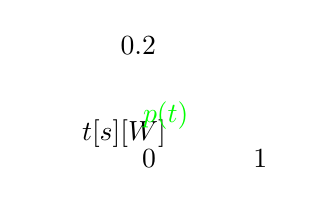
\begin{tikzpicture}[scale=1.2, samples=100, >=latex]
%%%%%%%%%%%%%%%%%%%%%%%%%%%%%%%%%%%%%%%%%%%%%%%%%%%%%%%%%%
\def\VoltageColor{blue!90!white}
\def\CurrentColor{red!90!white}
\def\PowerColor{green}
%%%%%%%%%%%%%%%%%%%%%%%%%%%%%%%%%%%%%%%%%%%%%%%%%%%%%%%%%%
\PlotGrid{-.1}{2}{-.2}{1.5}
\PlotAxes{-.2}{2.3}{-.2}{1.5}{$t [s]$}{$[W]$}
\draw (0,0) node[below left]{$0$};
\draw (0,1) node[left ]{$0.2$};
\draw (1,0) node[below]{$1$};
\draw (2,0) node[below]{$2$};
%%%%%%%%%%%%%%%%%%%%%%%%%%%%%%%%%%%%%%%%%%%%%%%%%%%%%%%%%%
\draw[color=\PowerColor, very thick] plot[id=powerVsTime_ex1, domain=0:2] function{5*10*x*(1-5*x)*exp(-10*x)} node[above] {$p(t)$};		
\end{tikzpicture}

\end{document}